Die erzeugten thermischen Neutronen %ref dazupacken auzs therorie
werden auf den Werkstoff gelenkt. Die anschließende auftretende Strahlung wir von dem Geiger-Müller-Zählrohr detektiert und mit den Zählern erfasst.
Durch die zwei Anzeigen der Zähler kann nun die ausgewertete Anzahl an Zerfällen abgelesen werden, während der Zeitgeber automatisch nach $\Delta t$ auf die Zweite Anzeige wechselt.
Dieser Vorgang wiederholt sich periodisch. Es lassen sich also ohne Pause genaue Messungen erzielen.

\begin{figure}
  \centering
  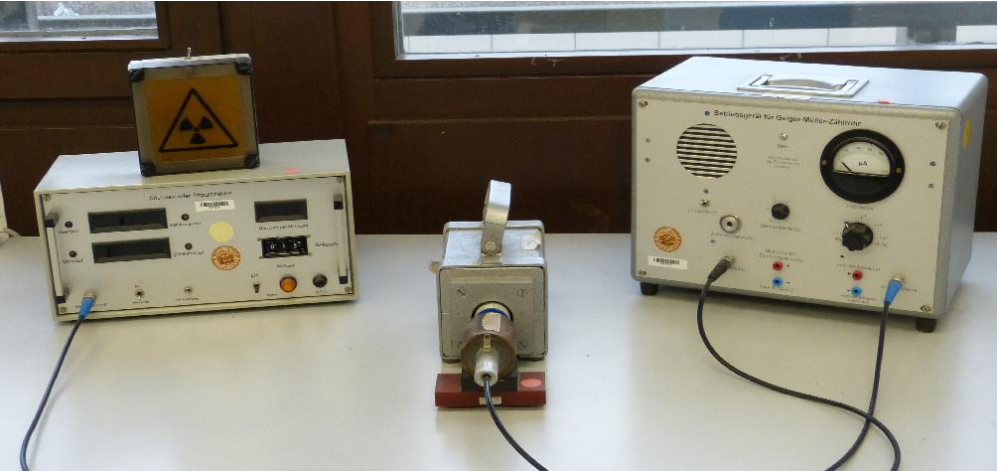
\includegraphics[width=0.8\textwidth]{bilder/Screenshot 2021-01-22 103203.png}
  \caption{Aufbau  \cite{hinweis}.}
  \label{fig:aufbau}
\end{figure}
Der Zeitgeber hat eine Genauigkeit von $10^{-5}$ auf das Gegebene Messintervall $\Delta t$.
Zusätzlich wird vor Beginn der Durchführung mit radioaktiven Substanzen der \textbf{Nulleffekt} $N_U$ %\ref zur theorie 
gemessen um ungewollte Strahlung nachher vom Ergebnis abziehen zu können.  Der Messung liegt ein statistischer Fehler bei, weswegen sich möglichst lange Messungen des Nulleffekts empfehlen.
\\
\newline
Beide Probem, Vanadium und Rhodium, werden unmittelbar nach der Aktivierung der Neutronen dem Geiger-Müller-Zählrohr zur Messung gegeben.
Die Intervalle untescheiden sich dahingehend, dass bei Vadium im Intervall von 30 Sekunden und bei Rhoidum im Intervall von 15 Sekunden gemessen wird.


